\documentclass{report}
\usepackage[a4paper,total={7in,10in}]{geometry}

\usepackage{amsmath}
\usepackage{amssymb}
\usepackage{enumitem}
\usepackage{tikz, pgfplots}
\usepackage{multicol}
\usepackage{setspace}
\usetikzlibrary{arrows}

\setcounter{chapter}{10}
\setcounter{section}{2}

\newcommand{\sol}{\vspace{1em}\\\textbf{Sol.}}
\newcommand{\eos}{ \qquad \square}

\begin{document}
\section*{Exercise 5b}

\onehalfspacing
\begin{enumerate}[leftmargin=*]
    \item Find the equation of the parabola of which its vertex is at point $(0, 0)$ and
          satisfies the following criteria:
          \begin{enumerate}
              \item The focus is at point $(0, 3)$. \sol{}
                    \begin{multicols}{2}
                        Since the vertex is at $(0, 0)$, the equation of the directrix is $y = -3$.

                        Let the coordinates of the moving point $P$ be $(x, y)$.

                        From the definition $|PF| = |PM|$,

                        we have
                        \begin{flalign*}
                            \sqrt{x^2 + (y-3)^2} & = |y - (-3)|   & \\
                            x^2 + (y-3)^2        & = (y+3)^2      & \\
                            x^2 + y^2 - 6y + 9   & = y^2 + 6y + 9 & \\
                            x^2                  & = 12y \eos
                        \end{flalign*}
                        \columnbreak
                        \pgfplotsset{ticks=none}
                        \begin{center}
                            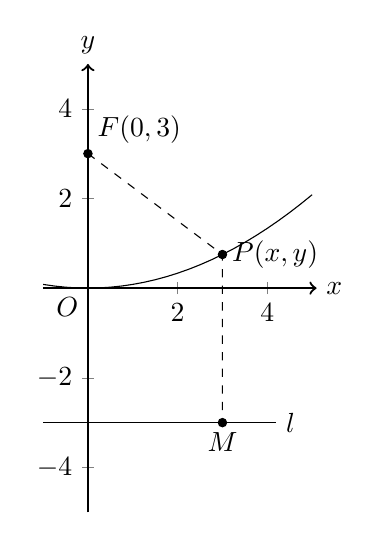
\begin{tikzpicture}
                                \begin{axis}[
                                        unit vector ratio*=1 1 1,
                                        xmin=-1,xmax=5.1,
                                        ymin=-5,ymax=5,
                                        axis lines=center,
                                        axis on top=true,
                                        domain=-1:5,
                                        axis lines=middle,
                                        axis line style={->, thick},
                                        xlabel=$x$,
                                        ylabel=$y$,
                                        every axis x label/.style={
                                                at={(ticklabel* cs:1)},
                                                anchor=west,
                                            },
                                        every axis y label/.style={
                                                at={(ticklabel* cs:1)},
                                                anchor=south,
                                            },
                                    ]
                                    \addplot [mark=none] {x^2/12};
                                    \addplot [mark=none, domain=-5:4.2] {-3};
                                    \node [right] at (axis cs:4.2, -3) {$l$};
                                    \draw [fill=black] (axis cs:0,3) circle (1.5pt);
                                    \node [above right] at (axis cs:0,3) {$F(0, 3)$};
                                    \draw [fill=black] (axis cs:3, 0.75) circle (1.5pt);
                                    \node [right] at (axis cs:3, 0.75) {$P(x, y)$};
                                    \draw [fill=black] (axis cs:3, -3) circle (1.5pt);
                                    \node [below] at (axis cs:3, -3) {$M$};
                                    \draw [dashed] (axis cs:0,3) -- (axis cs:3, 0.75) -- (axis cs:3, -3);
                                    \node [below left] at (axis cs:0,0) {$O$};
                                \end{axis}
                            \end{tikzpicture}
                        \end{center}
                    \end{multicols}
                    \vfill\null{}
              \item The directrix is $x - \dfrac{1}{4} = 0$. \sol{}
                    \begin{multicols}{2}
                        Since the vertex is at $(0, 0)$, the equation of the directrix is $x = \dfrac{1}{4}$

                        we know that the focus is at $\left(-\dfrac{1}{4}, 0\right)$.

                        Let the coordinates of the moving point $P$ be $(x, y)$.

                        From the definition $|PF| = |PM|$,

                        we have
                        \begin{flalign*}
                            \sqrt{\left(x + \frac{1}{4}\right)^2 + y^2} & = \left|x - \frac{1}{4}\right|      & \\
                            \left(x + \frac{1}{4}\right)^2 + y^2        & = \left(x - \frac{1}{4}\right)^2    & \\
                            x^2 + \frac{1}{2}x + \frac{1}{16} + y^2     & = x^2 - \frac{1}{2}x + \frac{1}{16} & \\
                            y^2                                         & = -x \eos
                        \end{flalign*}
                        \columnbreak
                        \pgfplotsset{ticks=none}
                        \begin{center}
                            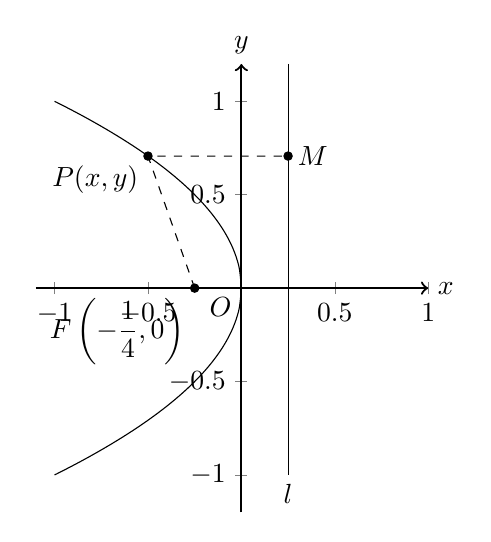
\begin{tikzpicture}
                                \begin{axis}[
                                        unit vector ratio*=1 1 1,
                                        xmin=-1.1,xmax=1,
                                        ymin=-1.2,ymax=1.2,
                                        axis lines=center,
                                        axis on top=true,
                                        domain=-1:0,
                                        axis lines=middle,
                                        axis line style={->, thick},
                                        xlabel=$x$,
                                        ylabel=$y$,
                                        every axis x label/.style={
                                                at={(ticklabel* cs:1)},
                                                anchor=west,
                                            },
                                        every axis y label/.style={
                                                at={(ticklabel* cs:1)},
                                                anchor=south,
                                            },
                                    ]
                                    \addplot [mark=none, smooth, samples=100] {(-x)^0.5};
                                    \addplot [mark=none, smooth, samples=100] {(-x)^0.5 * -1};
                                    \draw [fill=black] (axis cs:-0.25,0) circle (1.5pt);
                                    \node [below left] at (axis cs:-0.25,0) {$F\left(-\dfrac{1}{4}, 0\right)$};
                                    \draw (axis cs:0.25,1.2) -- (axis cs:0.25,-1);
                                    \node [below] at (axis cs:0.25,-1) {$l$};
                                    \draw [fill=black] (axis cs:-0.5, 0.707) circle (1.5pt) node [below left] {$P(x, y)$};
                                    \draw [fill=black] (axis cs:0.25, 0.707) circle (1.5pt) node [right] {$M$};
                                    \draw [dashed] (axis cs:-0.25,0) -- (axis cs:-0.5, 0.707) -- (axis cs:0.25, 0.707);
                                    \node [below left] at (axis cs:0,0) {$O$};
                                \end{axis}
                            \end{tikzpicture}
                        \end{center}
                    \end{multicols}
                    \vfill\null{}

                    \newpage
              \item Its focus is on the $x$-axis and passes through point $(5, -4)$. \sol{}

                    Since the focus is on the $x$-axis, we let the equation of the curve be $y^2 =
                        4ax$.

                    Substituting the coordinates of the point $(5, -4)$ into the equation, we have
                    \begin{flalign*}
                        (-4)^2 & = 4a(5)       & \\
                        16     & = 20a         & \\
                        a      & = \frac{4}{5}
                    \end{flalign*}
                    $\therefore$ the equation of the curve is $y^2 = \dfrac{16}{5}x$.

              \item Its focus is on the $y$-axis and passes through point $(-4, 2)$. \sol{}

                    Since the focus is on the $y$-axis, we let the equation of the curve be $x^2 =
                        4ay$.

                    Substituting the coordinates of the point $(-4, 2)$ into the equation, we have
                    \begin{flalign*}
                        (-4)^2 & = 4a(2) & \\
                        16     & = 8a    & \\
                        b      & = 2
                    \end{flalign*}
                    $\therefore$ the equation of the curve is $x^2 = 8y$.

              \item The distance from the vertex to the directrix is $2$. \sol{}

                    We have two scenarios:
                    \begin{multicols}{2}
                        \begin{enumerate}
                            \item The focus is on the $x$-axis.

                                  Since $|PF|=|PM|$, the foci are at $(\pm 1, 0)$, and the equations of the
                                  directrices are $x = \mp1$.

                                  Let the equations of the curves be $y^2 = 4ax$.

                                  Since the latus rectum is $|4\cdot (\pm1)| = 4$, the curves pass through $(\pm
                                      1, \pm 2)$.

                                  Substituting the coordinates of the point $(\pm 1, \pm 2)$ into the equation,
                                  we have we have
                                  \begin{flalign*}
                                      (\pm 2)^2 & = 4a(\pm 1) & \\
                                      4         & = \pm 4a    & \\
                                      a         & = \pm 1
                                  \end{flalign*}
                                  $\therefore$ the equation of the curve is $y^2 = \pm 4x$.

                            \item The focus is on the $y$-axis.

                                  Since $|PF|=|PM|$, the foci are at $(0, \pm 1)$, and the equations of the
                                  directrices are $y = \mp1$.

                                  Let the equations of the curves be $x^2 = 4ay$.

                                  Since the latus rectum is $|4\cdot (\pm1)| = 4$, the curves pass through $(\pm
                                      2, \pm 1)$.

                                  Substituting the coordinates of the point $(\pm 2, \pm 1)$ into the equation,
                                  we have we have
                                  \begin{flalign*}
                                      (\pm 2)^2 & = 4a(\pm 1) & \\
                                      4         & = \pm 4a    & \\
                                      a         & = \pm 1
                                  \end{flalign*}
                                  $\therefore$ the equation of the curve is $x^2 = \pm 4y$.
                        \end{enumerate}
                    \end{multicols}
          \end{enumerate}

          \newpage
    \item Find the coordinates of the focus point and the equation of the directrix of
          the following parabolas. Hence, sketch the graphs of the parabolas:
          \begin{enumerate}
              \item $2y^2 + 5x = 0$
                    \sol{}
                    \vspace{-3em}
                    \begin{multicols}{2}
                        \begin{flalign*}
                            2y^2 + 5x & = 0             & \\
                            y^2       & = -\frac{5}{2}x & \\
                            a         & = -\frac{5}{8}
                        \end{flalign*}
                        The coordinates of the focus point are $\left(-\dfrac{5}{8}, 0\right)$,

                        The equation of the directrices is $x = \dfrac{5}{8}$. \vfill\null{}
                        \pgfplotsset{ticks=none}
                        \begin{center}
                            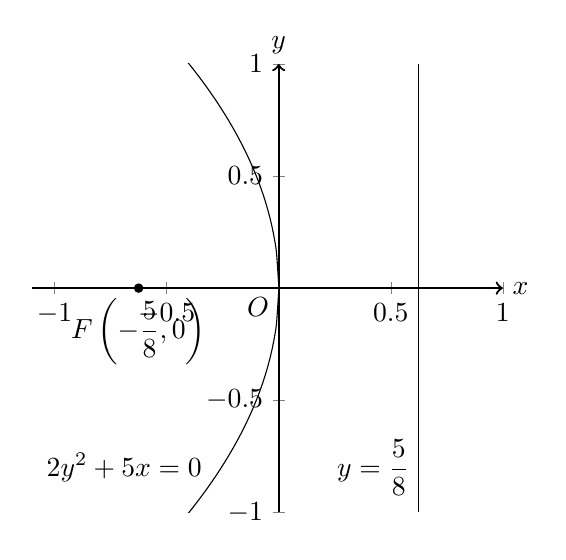
\begin{tikzpicture}
                                \begin{axis}[
                                        unit vector ratio*=1 1 1,
                                        xmin=-1.1,xmax=1,
                                        ymin=-1,ymax=1,
                                        axis lines=center,
                                        axis on top=true,
                                        domain=-1:0,
                                        axis lines=middle,
                                        axis line style={->, thick},
                                        xlabel=$x$,
                                        ylabel=$y$,
                                        every axis x label/.style={
                                                at={(ticklabel* cs:1)},
                                                anchor=west,
                                            },
                                        every axis y label/.style={
                                                at={(ticklabel* cs:1)},
                                                anchor=south,
                                            },
                                    ]
                                    \addplot [mark=none, smooth, samples=100] {(-5/2*x)^0.5};
                                    \addplot [mark=none, smooth, samples=100] {(-5/2*x)^0.5 * -1};
                                    \draw [fill=black] (axis cs:-5/8,0) circle (1.5pt);
                                    \node [below] at (axis cs:-5/8,0) {$F\left(-\dfrac{5}{8}, 0\right)$};
                                    \draw (axis cs:5/8,1) -- (axis cs:5/8,-1);
                                    \node [left] at (axis cs:5/8,-0.8) {$y=\dfrac{5}{8}$};
                                    \node [below left] at (axis cs:0,0) {$O$};
                                    \node [left] at (axis cs:-0.3,-0.8) {$2y^2 + 5x=0$};
                                \end{axis}
                            \end{tikzpicture}
                        \end{center}
                    \end{multicols}

              \item $x^2 - \dfrac{1}{2}y = 0$
                    \sol{}
                    \vspace{-3em}
                    \begin{multicols}{2}
                        \begin{flalign*}
                            x^2 - \frac{1}{2}y & = 0            & \\
                            x^2                & = \frac{1}{2}y & \\
                            a                  & = \frac{1}{8}
                        \end{flalign*}
                        The coordinates of the focus point are $\left(0, \dfrac{1}{8}\right)$,

                        The equation of the directrices is $y = -\dfrac{1}{8}$. \vfill\null{}
                        \pgfplotsset{ticks=none}
                        \begin{center}
                            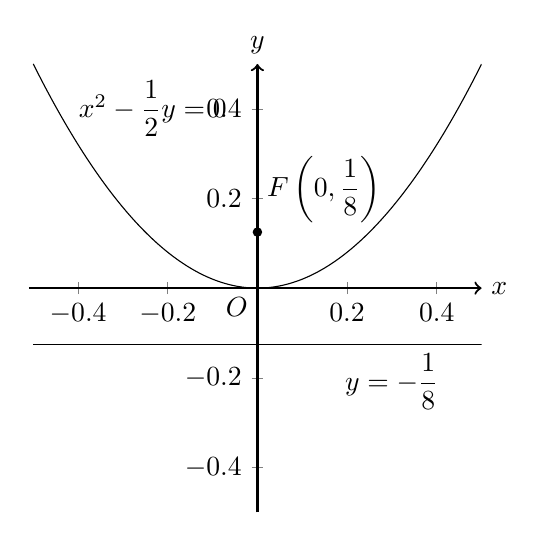
\begin{tikzpicture}
                                \begin{axis}[
                                        unit vector ratio*=1 1 1,
                                        xmin=-0.51,xmax=0.5,
                                        ymin=-0.5,ymax=0.5,
                                        axis lines=center,
                                        axis on top=true,
                                        domain=-0.5:0.5,
                                        axis lines=middle,
                                        axis line style={->, thick},
                                        xlabel=$x$,
                                        ylabel=$y$,
                                        every axis x label/.style={
                                                at={(ticklabel* cs:1)},
                                                anchor=west,
                                            },
                                        every axis y label/.style={
                                                at={(ticklabel* cs:1)},
                                                anchor=south,
                                            },
                                    ]
                                    \addplot [mark=none, smooth, samples=100] {2*x^2};
                                    \draw [fill=black] (axis cs:0,1/8) circle (1.5pt);
                                    \node [above right] at (axis cs:0,1/8) {$F\left(0, \dfrac{1}{8}\right)$};
                                    \draw (axis cs:-0.5,-1/8) -- (axis cs:0.5,-1/8);
                                    \node [below] at (axis cs:0.3,-1/8) {$y=-\dfrac{1}{8}$};
                                    \node [below left] at (axis cs:0,0) {$O$};
                                    \node [right] at (axis cs:-0.42,0.4) {$x^2 - \dfrac{1}{2}y = 0$};
                                \end{axis}
                            \end{tikzpicture}
                        \end{center}
                    \end{multicols}
          \end{enumerate}

    \item Find the coordinates of the vertex, the coordinates of the focus point, the
          axis of symmetry, the equation of the directrix, and the latus rectum of the
          following parabolas. Hence, sketch the graph.
          \begin{enumerate}
              \item $y^2 - 6x = 0$
                    \sol{}
                    \vspace{-3em}
                    \begin{multicols}{2}
                        \begin{flalign*}
                            y^2 - 6x & = 0                         & \\
                            y^2      & = 6x                        & \\
                            a        & = \frac{6}{4} = \frac{3}{2}
                        \end{flalign*}
                        The coordinates of the vertex are $(0, 0)$,

                        The coordinates of the focus point are $\left(\dfrac{3}{2}, 0\right)$,

                        The axis of symmetry is $y = 0$,

                        The equation of the directrices is $x = -\dfrac{3}{2}$,

                        The latus rectum is $\left|4\cdot \dfrac{3}{2}\right| = 6$. \columnbreak
                        \pgfplotsset{ticks=none}
                        \begin{center}
                            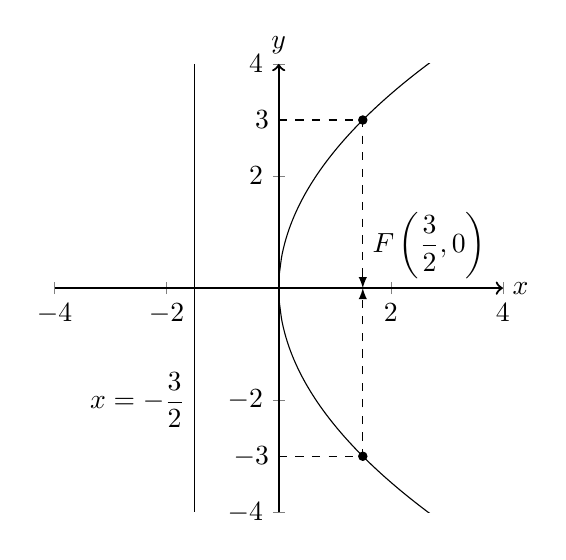
\begin{tikzpicture}
                                \begin{axis}[
                                        unit vector ratio*=1 1 1,
                                        xmin=-4,xmax=4,
                                        ymin=-4,ymax=4,
                                        axis lines=center,
                                        axis on top=true,
                                        domain=-1:3,
                                        axis lines=middle,
                                        axis line style={->, thick},
                                        xlabel=$x$,
                                        ylabel=$y$,
                                        every axis x label/.style={
                                                at={(ticklabel* cs:1)},
                                                anchor=west,
                                            },
                                        every axis y label/.style={
                                                at={(ticklabel* cs:1)},
                                                anchor=south,
                                            },
                                    ]
                                    \addplot [mark=none, smooth, samples=100] {(6*x)^0.5};
                                    \addplot [mark=none, smooth, samples=100] {(6*x)^0.5 * -1};
                                    \node [above right] at (axis cs:3/2,0) {$F\left(\dfrac{3}{2}, 0\right)$};
                                    \draw (axis cs:-3/2,4) -- (axis cs:-3/2,-4);
                                    \node [left] at (axis cs:-3/2,-2) {$x=-\dfrac{3}{2}$};
                                    \draw [fill=black] (axis cs:1.5,3) circle (1.5pt);
                                    \draw [fill=black] (axis cs:1.5,-3) circle (1.5pt);
                                    \draw [-latex, dashed] (axis cs:0,3) -- (axis cs:1.5,3) -- (axis cs:3/2,0);
                                    \draw [-latex, dashed] (axis cs:0,-3) -- (axis cs:1.5,-3) -- (axis cs:3/2,0);
                                    \node [left] at (axis cs:0, 3) {$3$};
                                    \node [left] at (axis cs:0, -3) {$-3$};
                                \end{axis}
                            \end{tikzpicture}
                        \end{center}
                    \end{multicols}
              \item $4x^2 + 3y = 0$
                    \sol{}
                    \vspace{-3em}
                    \begin{multicols}{2}
                        \begin{flalign*}
                            4x^2 + 3y & = 0             & \\
                            x^2       & = -\frac{3}{4}y & \\
                            a         & = -\frac{3}{16}
                        \end{flalign*}
                        The coordinates of the vertex are $(0, 0)$,

                        The coordinates of the focus point are $\left(0, -\dfrac{3}{16}\right)$,

                        The axis of symmetry is $x = 0$,

                        The equation of the directrices is $y = \dfrac{3}{16}$,

                        The latus rectum is $\left|4\cdot \left(-\dfrac{3}{16}\right)\right| =
                            \dfrac{3}{4}$. \columnbreak \pgfplotsset{ticks=none}
                        \begin{center}
                            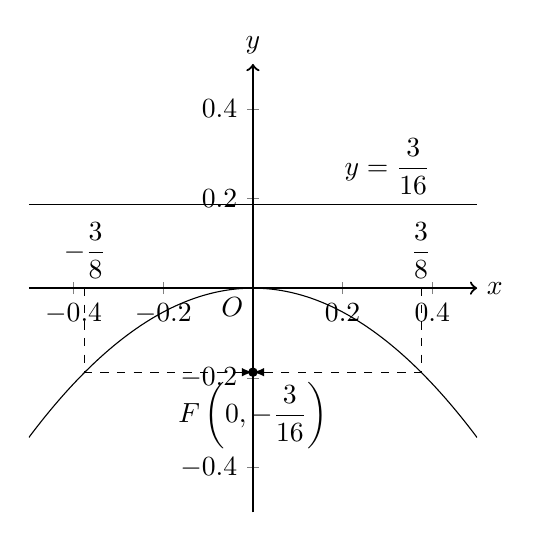
\begin{tikzpicture}
                                \begin{axis}[
                                        unit vector ratio*=1 1 1,
                                        xmin=-0.5,xmax=0.5,
                                        ymin=-0.5,ymax=0.5,
                                        axis lines=center,
                                        axis on top=true,
                                        domain=-0.5:0.5,
                                        axis lines=middle,
                                        axis line style={->, thick},
                                        xlabel=$x$,
                                        ylabel=$y$,
                                        every axis x label/.style={
                                                at={(ticklabel* cs:1)},
                                                anchor=west,
                                            },
                                        every axis y label/.style={
                                                at={(ticklabel* cs:1)},
                                                anchor=south,
                                            },
                                    ]
                                    \addplot [mark=none, smooth, samples=100] {-4/3*x^2};
                                    \draw [fill=black] (axis cs:0,-3/16) circle (1.5pt);
                                    \node [below] at (axis cs:0,-3/16) {$F\left(0, -\dfrac{3}{16}\right)$};
                                    \draw (axis cs:-0.5,3/16) -- (axis cs:0.5,3/16);
                                    \node [above] at (axis cs:0.3,3/16) {$y=\dfrac{3}{16}$};
                                    \draw [-latex, dashed] (axis cs:-3/8, 0) -- (axis cs:-3/8, -3/16) -- (axis cs:0, -3/16);
                                    \draw [-latex, dashed] (axis cs:3/8, 0) -- (axis cs:3/8, -3/16) -- (axis cs:0, -3/16);
                                    \node [above] at (axis cs:-3/8, 0) {$-\dfrac{3}{8}$};
                                    \node [above] at (axis cs:3/8, 0) {$\dfrac{3}{8}$};
                                    \node [below left] at (axis cs:0,0) {$O$};
                                \end{axis}
                            \end{tikzpicture}
                        \end{center}
                    \end{multicols}
              \item $y^2 + 4x - 4y = 0$
                    \sol{}
                    \vspace{-3em}
                    \begin{multicols}{2}
                        \begin{flalign*}
                            y^2 + 4x - 4y & = 0         & \\
                            y^2 - 4y      & = -4x       & \\
                            y^2 - 4y + 4  & = -4x + 4   & \\
                            (y - 2)^2     & = -4(x - 1)
                        \end{flalign*}
                        Let $y' = y - 2$, $x' = x - 1$, we have $(y')^2 = -4x'$.

                        The coordinates of the vertex are $(0, 0)$,

                        The coordinates of the focus point are $\left(-1, 0\right)$,

                        The axis of symmetry is $y' = 0$,

                        The equation of the directrices is $y' = 1$,\\

                        In the original equation,

                        The coordinates of the vertex are $\left\{\begin{array}{l} 0 = x - 1 \\ 0 = y - 2
                            \end{array}\right.$, i.e. $(1, 2)$,

                        The coordinates of the focus point are $\left\{\begin{array}{l} -1 = x - 1 \\ \hspace{0.8em}0 = y - 2
                            \end{array}\right.$, i.e. $(0, 2)$,

                        The axis of symmetry is $0 = y - 2$, i.e. $y = 2$,

                        The equation of the directrices is $1 = x - 1$, i.e. $x = 2$,

                        The latus rectum is $\left|4\cdot (-1)\right| = 4$. \columnbreak
                        \pgfplotsset{ticks=none}
                        \begin{center}
                            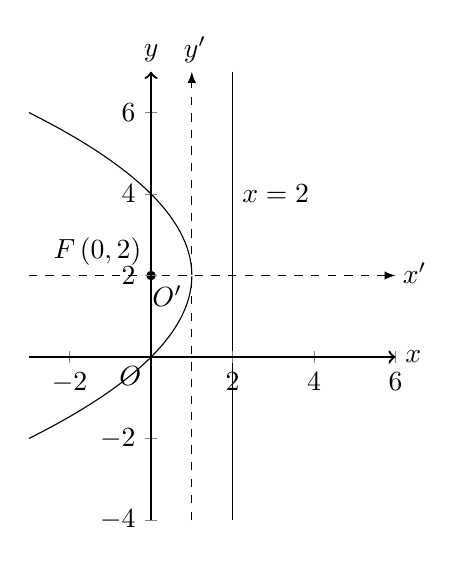
\begin{tikzpicture}
                                \begin{axis}[
                                        unit vector ratio*=1 1 1,
                                        xmin=-3,xmax=6,
                                        ymin=-4,ymax=7,
                                        axis lines=center,
                                        axis on top=true,
                                        domain=-3:1,
                                        axis lines=middle,
                                        axis line style={->, thick},
                                        xlabel=$x$,
                                        ylabel=$y$,
                                        every axis x label/.style={
                                                at={(ticklabel* cs:1)},
                                                anchor=west,
                                            },
                                        every axis y label/.style={
                                                at={(ticklabel* cs:1)},
                                                anchor=south,
                                            },
                                    ]
                                    \addplot [mark=none, smooth, samples=1000] {2 + (-4*x + 4)^0.5};
                                    \addplot [mark=none, smooth, samples=1000] {2 + (-4*x + 4)^0.5 * -1};
                                    \draw [-latex,dashed] (axis cs:1,-4) -- (axis cs:1,7);
                                    \draw [-latex,dashed] (axis cs:-3,2) -- (axis cs:6,2);
                                    \draw (axis cs:2,7) -- (axis cs:2,-4);
                                    \node [right] at (axis cs:2,4) {$x=2$};
                                    \draw [fill=black] (axis cs:0,2) circle (1.5pt) node [above left] {$F\left(0, 2\right)$};
                                    \node [below left] at (axis cs:0,0) {$O$};
                                    \node [below left] at (axis cs:1,2) {$O'$};
                                \end{axis}
                                \node at (2.11, 5.97) {$y'$};
                                \node at (4.9, 3.14) {$x'$};
                            \end{tikzpicture}
                        \end{center}
                    \end{multicols}
                    \newpage
              \item $x^2 - 4x - y + 5 = 0$
                    \sol{}
                    \vspace{-3em}
                    \begin{multicols}{2}
                        \begin{flalign*}
                            x^2 - 4x - y + 5     & = 0     & \\
                            x^2 - 4x + 4 - y + 5 & = 4     & \\
                            (x - 2)^2            & = y - 1
                        \end{flalign*}
                        Let $x' = x - 2$, $y' = y - 1$, we have $(x')^2 = y'$.

                        The coordinates of the vertex are $(0, 0)$,

                        The coordinates of the focus point are $\left(0, \dfrac{1}{4}\right)$,

                        The axis of symmetry is $x' = 0$,

                        The equation of the directrices is $x' = -\dfrac{1}{4}$,\\

                        In the original equation,

                        The coordinates of the vertex are $\left\{\begin{array}{l} 0 = x - 2 \\ 0 = y - 1
                            \end{array}\right.$, i.e. $(2, 1)$,

                        The coordinates of the focus point are $\left\{\begin{array}{l} 0 = x - 2 \\ \dfrac{1}{4} = y - 1
                            \end{array}\right.$, i.e. $\left(2, \dfrac{5}{4}\right)$,

                        The axis of symmetry is $0 = x - 2$, i.e. $x = 2$,

                        The equation of the directrices is $-\dfrac{1}{4} = y - 1$, i.e. $y =
                            \dfrac{3}{4}$,

                        The latus rectum is $\left|4\cdot \dfrac{1}{4}\right| = 1$. \columnbreak

                        \pgfplotsset{ticks=none}
                        \begin{center}
                            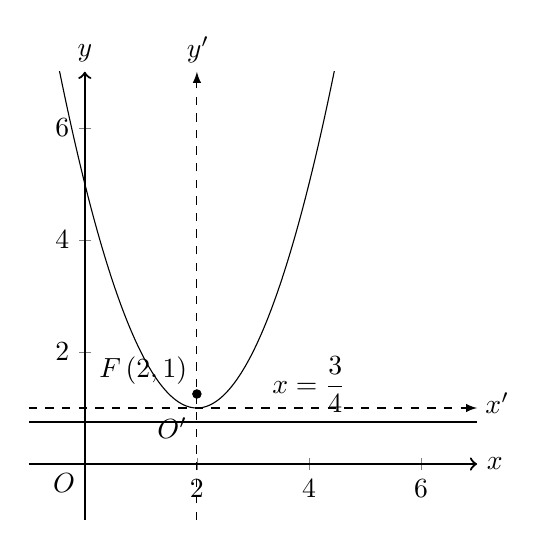
\begin{tikzpicture}
                                \begin{axis}[
                                        unit vector ratio*=1 1 1,
                                        xmin=-1,xmax=7,
                                        ymin=-1,ymax=7,
                                        axis lines=center,
                                        axis on top=true,
                                        domain=-1:7,
                                        axis lines=middle,
                                        axis line style={->, thick},
                                        xlabel=$x$,
                                        ylabel=$y$,
                                        every axis x label/.style={
                                                at={(ticklabel* cs:1)},
                                                anchor=west,
                                            },
                                        every axis y label/.style={
                                                at={(ticklabel* cs:1)},
                                                anchor=south,
                                            },
                                    ]
                                    \addplot [mark=none, smooth, samples=1000] {(x-2)^2 + 1};
                                    \draw [-latex,dashed] (axis cs:-1,1) -- (axis cs:7,1);
                                    \draw [-latex,dashed] (axis cs:2,-1) -- (axis cs:2,7);
                                    \draw (axis cs:-1,0.75) -- (axis cs:7,0.75);
                                    \node [above] at (axis cs:4,0.75) {$x=\dfrac{3}{4}$};
                                    \draw [fill=black] (axis cs:2,1.25) circle (1.5pt) node [above left] {$F\left(2, 1\right)$};
                                    \node [below left] at (axis cs:0,0) {$O$};
                                    \node [below left] at (axis cs:2,1) {$O'$};
                                \end{axis}
                                \node at (2.15, 5.97) {$y'$};
                                \node at (5.95, 1.48) {$x'$};
                            \end{tikzpicture}
                        \end{center}
                    \end{multicols}
          \end{enumerate}

    \item The distance between a point on the parabola $y^2 = 12x$ and its focus point is
          $9$, find the coordinates of this point. \sol{}

          The vertex of the parabola is $(0, 0)$, the focus point is $(3, 0)$. Let the
          point be $\left(\dfrac{y^2}{12}, y\right)$, then
          \begin{flalign*}
              \sqrt{\left(\dfrac{y^2}{12} - 3\right)^2 + y^2}       & = 9                                            & \\
              \dfrac{y^4}{144} - \dfrac{y^2}{2} + 9 + y^2           & = 81                                           & \\
              \dfrac{y^4}{144} + \dfrac{y^2}{2}                     & = 72                                           & \\
              y^4 + 72y^2 - 10368                                   & = 0                                            & \\
              (y^2 + 144)(y^2 - 72)                                 & = 0                                            & \\
              y^2                                             = 72  & \text{ or } y^2 = -144 (\text{ rejected})      & \\
              y                                               = \pm & 6\sqrt{2}                                      & \\
              x                                                     & = \dfrac{\left(\pm 6\sqrt{2}\right)^2}{12} = 6
          \end{flalign*}
          Therefore, the coordinates of the point are $\left(6, \pm6\sqrt{2}\right)$.

    \item Find the equation of the parabola that has the vertex of $(3, -2)$ and the
          directrix of $y+8=0$. Hence, sketch the graph of the parabola. \sol{}

          \begin{multicols}{2}
              Let the equation of the parabola be $(x-3)^2 = 4a(y+2)$.

              Let $x' = x - 3$, $y' = y + 2$, we have $(x')^2 = 4ay'$.

              The equation of the directrix is $y = -8\ \cdots\ (1)$,

              $y+2 = y'$, $y = y' - 2\ \cdots\ (2)$

              Substituting $(1)$ into $(2)$,
              \begin{flalign*}
                  y' - 2 & = -8 & \\
                  y' + 6 & = 0
              \end{flalign*}

              Hence, $a = 6$

              Therefore, the equation of the parabola is
              \begin{flalign*}
                  (x-3)^2             & = 24(y+2)  & \\
                  x^2 - 6x + 9        & = 24y + 48   \\
                  x^2 - 6x - 24y - 39 & = 0 \eos
              \end{flalign*}

              The coordinates of the focus point are $\left\{\begin{array}{l} 0 = x - 3 \\6 = y + 2
                  \end{array}\right.$, i.e. $(3, 4)$,

              \columnbreak

              \pgfplotsset{ticks=none}
              \begin{center}
                  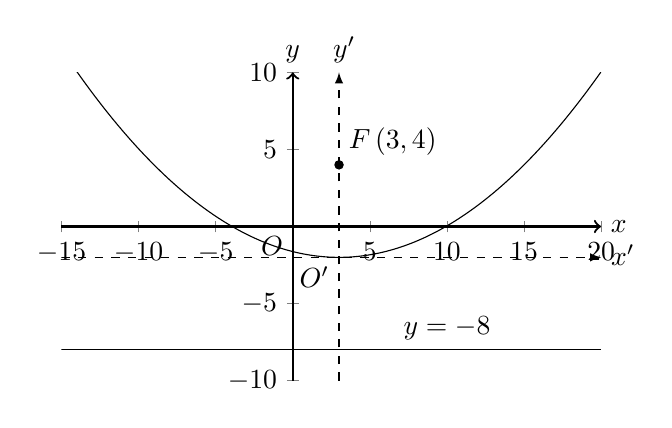
\begin{tikzpicture}
                      \begin{axis}[
                              unit vector ratio*=1 1 1,
                              xmin=-15,xmax=20,
                              ymin=-10,ymax=10,
                              axis lines=center,
                              axis on top=true,
                              domain=-15:20,
                              axis lines=middle,
                              axis line style={->, thick},
                              xlabel=$x$,
                              ylabel=$y$,
                              every axis x label/.style={
                                      at={(ticklabel* cs:1)},
                                      anchor=west,
                                  },
                              every axis y label/.style={
                                      at={(ticklabel* cs:1)},
                                      anchor=south,
                                  },
                          ]
                          \addplot [mark=none, smooth, samples=1000] {(x-3)^2/24 - 2};
                          \draw [-latex,dashed] (axis cs:-15,-2) -- (axis cs:20,-2);
                          \draw [-latex,dashed] (axis cs:3,-10) -- (axis cs:3,10);
                          \draw (axis cs:-15,-8) -- (axis cs:20,-8);
                          \node [above] at (axis cs:10,-8) {$y=-8$};
                          \draw [fill=black] (axis cs:3,4) circle (1.5pt) node [above right] {$F\left(3, 4\right)$};
                          \node [below left] at (axis cs:0,0) {$O$};
                          \node [below left] at (axis cs:3,-2) {$O'$};
                      \end{axis}
                      \node at (3.59, 4.2) {$y'$};
                      \node at (7.13, 1.6) {$x'$};
                  \end{tikzpicture}
              \end{center}
          \end{multicols}
\end{enumerate}
\end{document}